\documentclass[12pt]{article}
\usepackage{fullpage}
\usepackage{nopageno}
\usepackage{add-copyright}

\usepackage{amssymb}
\newcommand{\R}{\mathbb{R}}
\newcommand{\N}{\mathbb{N}}

\usepackage{graphicx}

\title{Midterm 2 Results}

\begin{document}

\section*{Results for Midterm 2}

The quartiles fell as follows:
\begin{center}
25\% of you scored above 202. \\
50\% of you scored above 192. \\
75\% of you scored above 177.
\end{center}
The median was 192.  The mean was 189.  The standard deviation was 15.
Here is the breakdown per problem:
\begin{center}
\begin{tabular}{lll}
\textbf{Problem} & \textbf{Average Score} & \textbf{Technique} \\
\hline
Problem 10 & 70.5\% & Power series convergence by comparison \\
Problem 6  & 71.8\% & Taylor series for $\sinh$ \\
Problem 11 & 72.1\% & Differentiate power series \\
Problem 8  & 74.5\% & Lagrange's theorem \\
Problem 12 & 76.1\% & Extra Credit \\
Problem 5  & 79.9\% & Taylor series $\cos \sin x$\\
Problem 2  & 82.6\% & Limit comparison and $n$-th term test \\
Problem 4  & 84.8\% & Absolute and conditional convergence \\
Problem 7  & 85.6\% & Taylor's theorem \\
Problem 9  & 93.2\% & Power series convergence by ratio test \\
Problem 1  & 93.3\% & Definition of convergence\\
Problem 3  & 95.3\% & Definition of ratio test
\end{tabular}
\end{center}

\subsection*{Relationship between the midterms}

The scores from the second exam do correlate with the scores from the
first exam; the normalized scores on the second midterm were about
70\% those of the first midterm.  Here is a formula relating the
second midterm scores to the first midterm scores:
$$
\mbox{Second  Midterm} = 0.682 \cdot \mbox{First Midterm} + 47.8
$$
For example, if I scored 210 on the first midterm, I might have
expected to score 191 on the second midterm.

\subsection*{Translation into letter grades}

If the sum of your scores on the midterms exceeds 400, you are on
track to get an \textbf{A}.  Scoring above 350 points puts you on
target for a \textbf{B}.

If you are not doing as well as you want to be doing, you should talk
to me so we can work together towards your success. I have weighted
the final exam heavily not because I want the final exam to be
terrifying, but because I want to give you every opportunity to pull
your grade up.

\pagebreak

\subsection*{An inspirational message}

There can be some concern about how I will be assigning letter grades.
I take the assignment of grades extremely seriously: the numbers I
give out frankly don't matter, but the letter grades I give out will
be on your college transcript forever.  I will do my best to be both
merciful and just (as I hope I have demonstrated during the quarter).

It was not so long ago that I received grades, and for all the effort
I put into my grades, they have proved to be unimportant.
Recommendation letters, on the other hand, are extremely important, as
is hard work.

Hard work is most important of all. You may find things are easy now,
but there will come a time when mathematics will be hard (we humans
are fortunate to be able to do any mathematics at all), and what
distinguishes the merely talented from the truly great is not skill,
but persistence.

\subsection*{The definition of mathematics is discipline}

Looking up $\mu \alpha \theta\ldots$ in a Greek-English lexicon:
\begin{center}
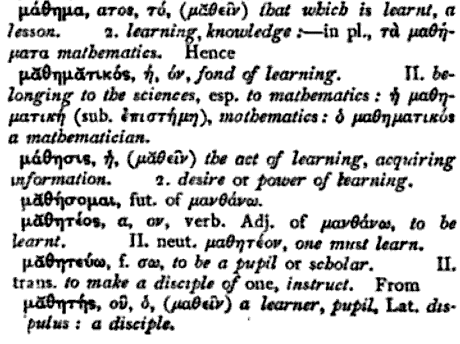
\includegraphics[width=3.5in]{math-definition.png}
\end{center}
Indeed, mathematics epitomizes learning.

\end{document}
